\pdfminorversion=4
\documentclass[aspectratio=169]{beamer}
\usepackage{verbatim}
\newenvironment{metaverbatim}{\verbatim}{\endverbatim}
\usepackage{courier}
\usepackage{lmodern}
\usepackage{apacite}
\usepackage[hidelinks]{hyperref}
\usepackage{xcolor}
\xdefinecolor{azulcesafuerte}{HTML}{14387e}
\xdefinecolor{azulcesaclaro}{HTML}{7ab6e0}
\xdefinecolor{azulcesamedio}{HTML}{0A72BC}

\usetheme{Madrid}
%\usecolortheme[named=black]{structure}
%
\setbeamercolor{normal text}{fg=azulcesafuerte}
\setbeamercolor{background canvas}{bg=white}
\setbeamercolor{frametitle}{fg=white, bg=azulcesafuerte}
\setbeamercolor{block title}{bg=azulcesafuerte,fg=azulcesaclaro}
\setbeamercolor{navigation symbols}{}

\setbeamertemplate{background}{\tikz[overlay,remember picture]\node[opacity=0.15]at (current page.center){\includegraphics[width=6.5cm]{}};}
\usepackage{tikz}
\usepackage{kantlipsum}
\setbeamercolor*{title}{fg=white, bg=azulcesafuerte}
\setbeamercolor{titlelike}{parent=structure}

\setbeamercolor*{palette primary}{bg=azulcesafuerte,fg=white}
\setbeamercolor*{palette secondary}{bg=azulcesafuerte,fg=white}
\setbeamercolor*{palette tertiary}{bg=azulcesafuerte,fg=white}

% Change base colour beamer@blendedblue (originally RGB: 0.2,0.2,0.7)
\colorlet{beamer@blendedblue}{azulcesaclaro}
\usepackage[spanish]{babel}
\usepackage{apacite}
\usepackage{marvosym}
\usepackage{subfig}
\usepackage{graphicx}
\usepackage[utf8x]{inputenc}
\usepackage{url}
\usepackage{hyperref}
\usepackage{times}
\usepackage{pxfonts}
\usepackage{fontenc}
%\usepackage[dvipsnames]{xcolor}
\setbeamertemplate{bibliography item}[text]
\title[Fundamentos de Analítica de Datos: Caso 1]{Fundamentos de Analítica de Datos: Caso 1}
\subtitle{(Sesión 6B)}

\author[Prof. Juan C. Correa, Ph.D.]{Prof. Juan C. Correa, Ph.D.}

\institute[]{
Colegio de Estudios Superiores de Administración\\
Bogotá - Colombia\\
% \color{azulcesaclaro}\Email  \href{mailto:juan.correan@cesa.edu.co}{juan.correan@cesa.edu.co}
}
\pgfdeclareimage[height=0.6cm]{OL}{OL}
 \logo{\pgfuseimage{OL}}
 \setbeamertemplate{caption}[numbered]
\date[Bogotá, Agosto, 2021] % (optional)
{}

\subject{}
\begin{document}
\begin{frame}
\titlepage
\end{frame}

% \begin{frame}
% \frametitle{Agenda} 
% \tableofcontents
% \end{frame}

\begin{frame}
\begin{block}{Objetivo de Aprendizaje}
En la Sesión 6A, se enseñaron algunos de los fundamentos del pre-procesamiento y la
visualización de datos. Al finalizar esta sesión y la siguiente (sesión 7A), usted estará en
capacidad de profundizar aún más en la visualización de datos con Pandas, Matplotlib y
ggplot2.
\end{block}
\end{frame}

\section{Insumos Preliminares}
\begin{frame}
\begin{center}
\Huge
\textcolor{azulcesaclaro}{1\\
--------------------------------\\
Insumos Preliminares}
\end{center}
\end{frame}

\begin{frame}
Para esta sesión, usted continuará usando el mismo repositorio de GitHub que clonamos para la sesión 6A. Si no lo ha hecho aún, acá tiene el enlace.
\begin{figure}
\centering
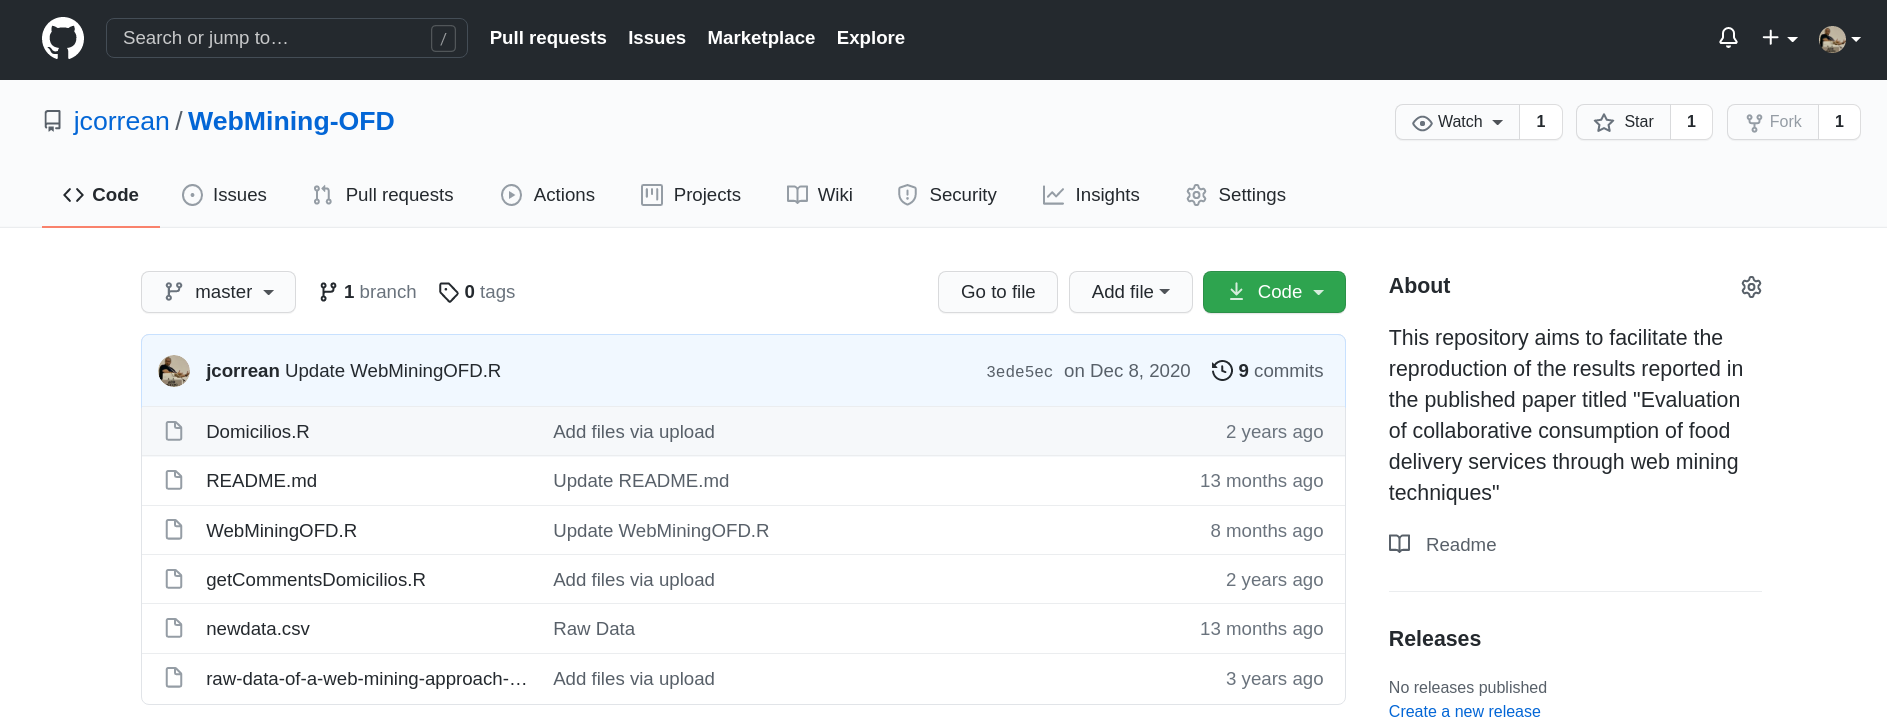
\includegraphics[width=.85\textwidth]{github1.png}
\end{figure}
\centering
\textcolor{blue}{\url{https://github.com/jcorrean/WebMining-OFD}}
\end{frame}

\section{Fundamentos de Pre-procesamiento de Datos}
\begin{frame}
\begin{center}
\Huge
\textcolor{azulcesaclaro}{2\\
--------------------------------\\
Fundamentos de Pre-procesamiento de Datos\\
(Continuación)}
\end{center}
\end{frame}

\begin{frame}
En la sesión 6A (slide 10) afirmamos que el futuro  gerente de una \textbf{empresa data-driven} debe entender en qué consiste el trabajo de un experto en analítica de datos.\\
\begin{figure}
\centering
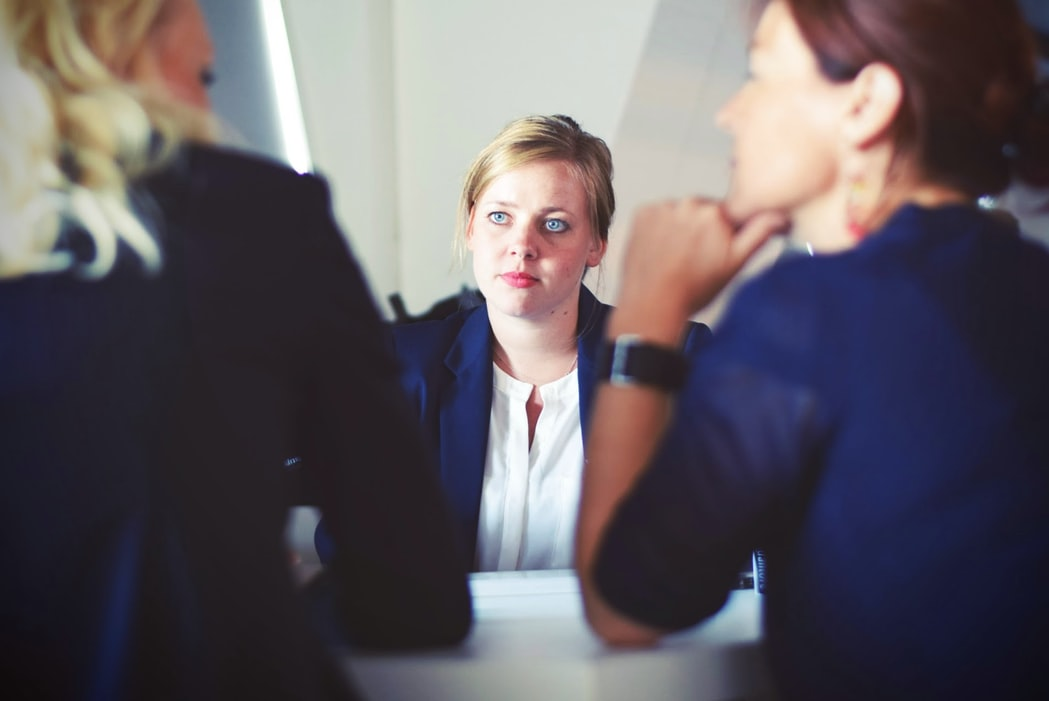
\includegraphics[width=.35\textwidth]{selection.jpeg}
\end{figure}
La razón que sustenta esa idea es que usted tendrá que decidir entre contratar empleados con experiencia o seleccionar proveedores expertos en analítica de datos. En cualquier caso, su decisión será acertada si y solo si usted sabe detectar esos criterios de experticia.
\end{frame}

\begin{frame}
Incluso, en el ámbito del emprendimiento es fundamental entender la visión de los expertos en analítica de datos \cite{Kotha2014}. ¿Por qué?
\begin{figure}
\centering
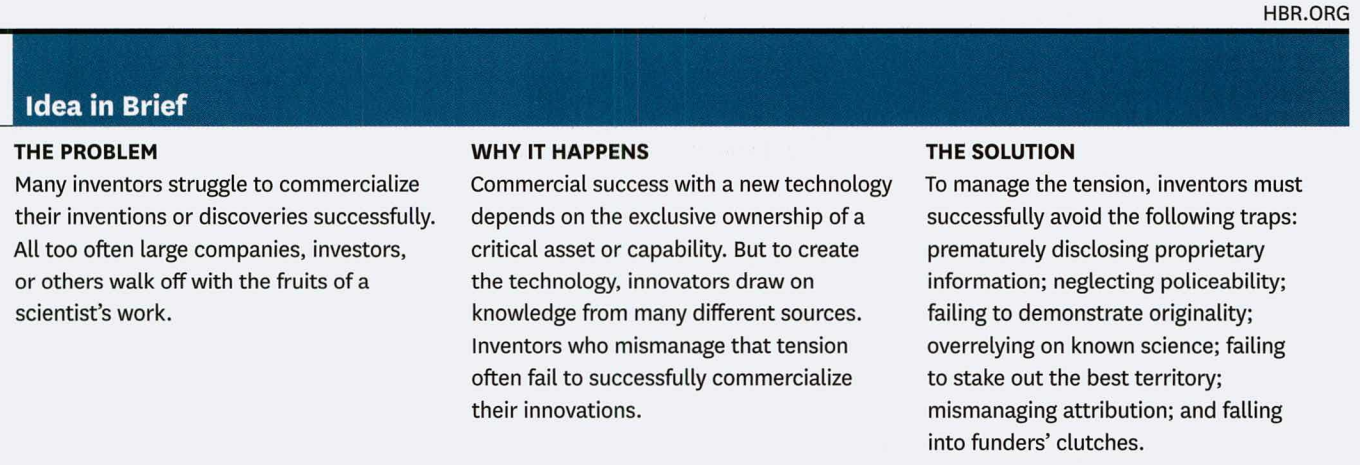
\includegraphics[width=.85\textwidth]{Kotha.png}
\end{figure}
Porque un experto en analítica de datos es un profesional con un sólido entrenamiento en ciencias (e.g., estadística, matemáticas, física, computación).
\end{frame}

\begin{frame}
En la sesión 6A (slide 6) afirmamos que el \textbf{el pre-procesamiento de datos} comprendía a todas las actividades que preceden al análisis de los datos. 
\begin{figure}
\centering
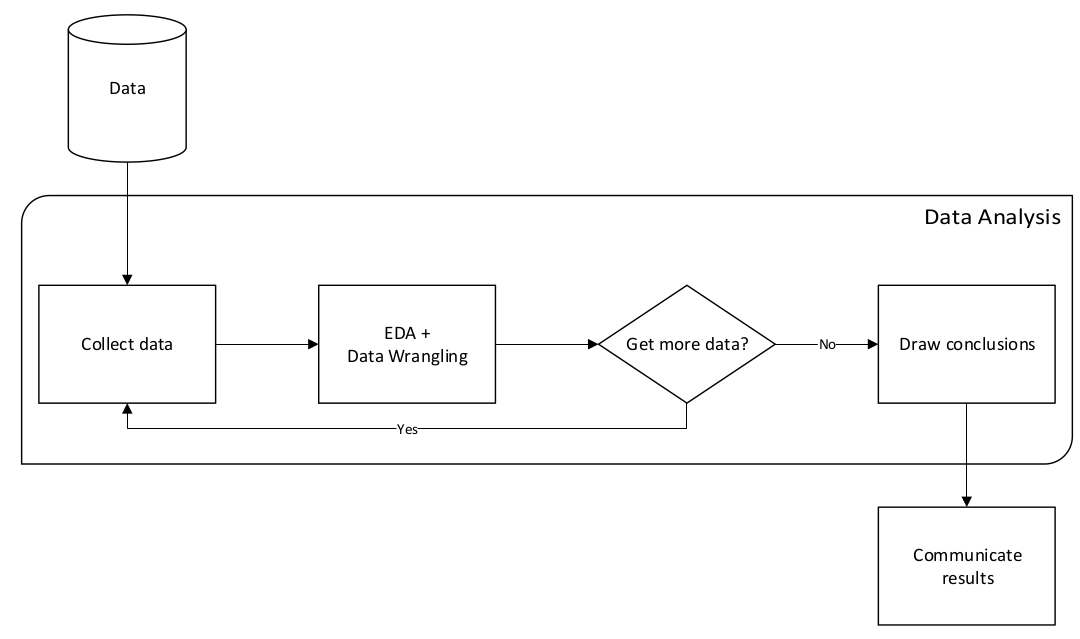
\includegraphics[width=.55\textwidth]{DAW.png}
\end{figure}
Para \citeauthor{Molin2021} \citeyear{Molin2021} esas actividades son Data, collect data, y EDA + Data Wrangling.
\end{frame}

\begin{frame}
Para \citeauthor{Wickham2017} \citeyear{Wickham2017} las actividades de pre-procesamiento implicarían Import, Tidy, Transform y Visualize, a excepción de model y communicate.
\begin{figure}
\centering
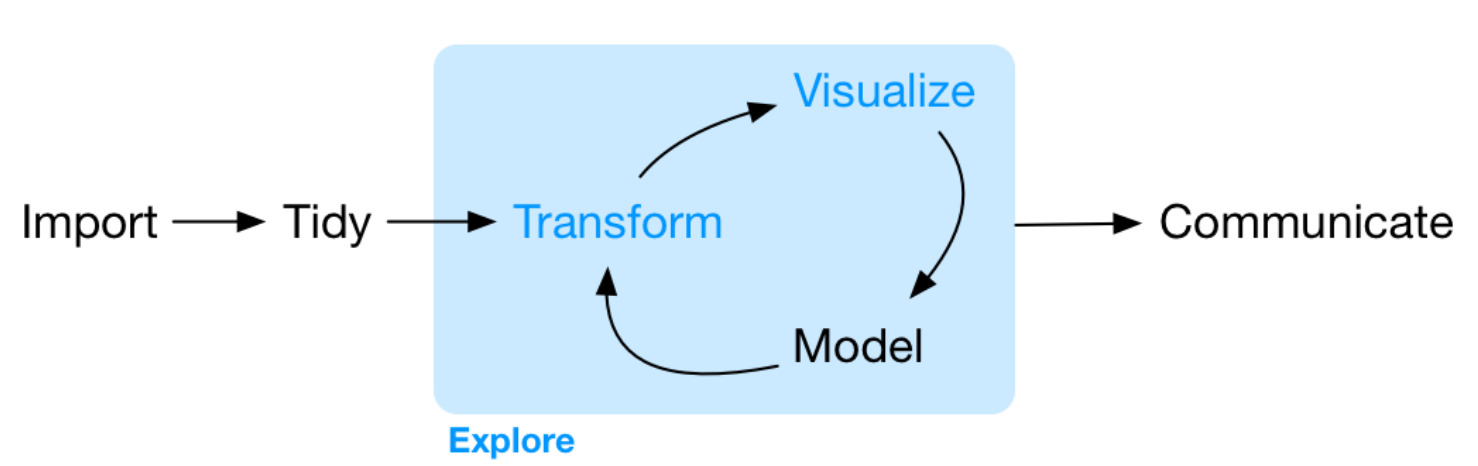
\includegraphics[width=.8\textwidth]{DE.png}
\end{figure}
\end{frame}



\begin{frame}
Para \citeauthor{Shmueli2020} \citeyear{Shmueli2020} el pre-procesamiento implica Data Preparation, Exploration, and Reduction.

\begin{figure}
\centering
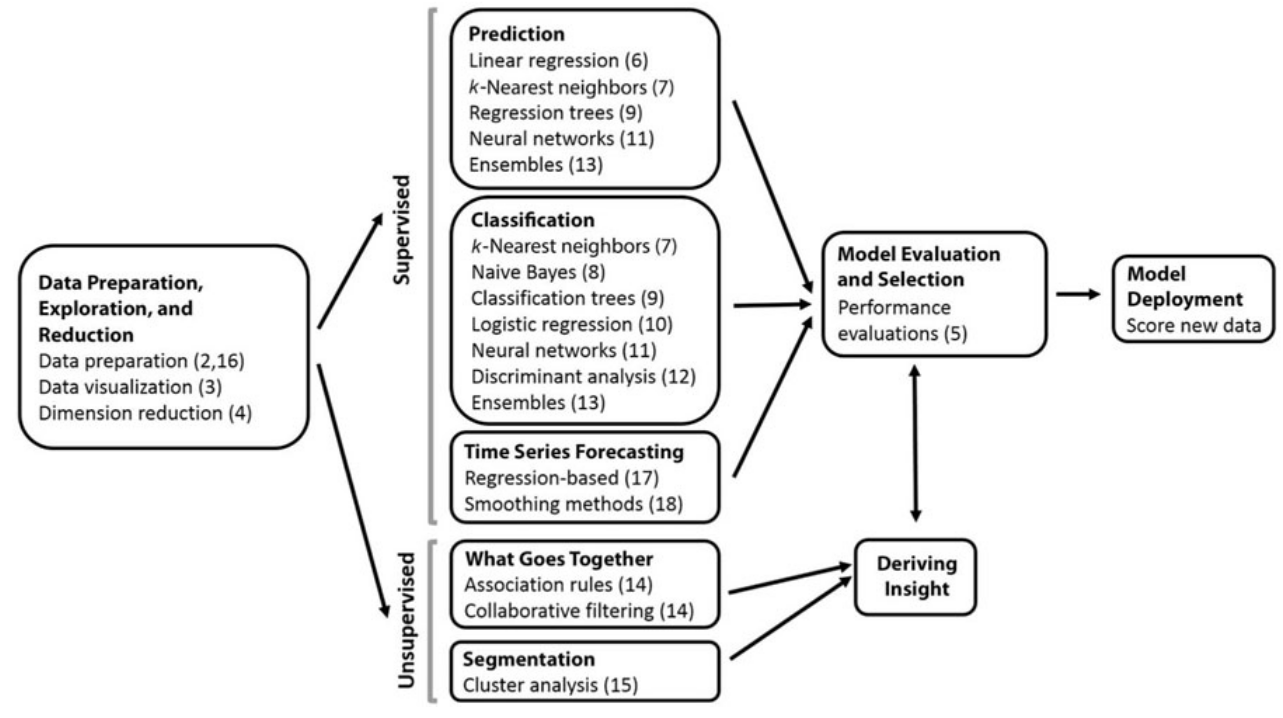
\includegraphics[width=.65\textwidth]{DM.png}
\end{figure}
\end{frame}

\begin{frame}
Ejercicio guiado:\\
\vspace{0.3cm}

\begin{itemize}
\item Equipo 1: Consultar en el libro de \citeauthor{Molin2021} \citeyear{Molin2021} 
\item Equipo 2: Consultar en el libro de \citeauthor{Wickham2017} \citeyear{Wickham2017}
\item Equipo 3: Consultar en el libro de \citeauthor{Shmueli2020} \citeyear{Shmueli2020}
\end{itemize}
\vspace{0.3cm}
Responder a las siguientes preguntas, luego de analizar concienzudamente la tabla de contenidos del libro
\begin{itemize}
\vspace{0.3cm}
\item ¿Cuáles y cuántos capítulos corresponden a pre-procesamiento?
\item ¿Cuántas páginas tiene cada capítulo?
\item ¿Cuántas sintaxis específicas aparecen en los capítulos que corresponden a pre-procesamiento?
\end{itemize}
\end{frame}

\section{Fundamentos de Análisis de Datos}
\begin{frame}
\begin{center}
\Huge
\textcolor{azulcesaclaro}{3\\
--------------------------------\\
Fundamentos de Análisis de Datos}
\end{center}
\end{frame}

\begin{frame}
Retomemos el script que habíamos estudiado en el slide 8 de Sesión 6A (cuya demostración se hizo en clase usando R). Vamos a concentrarnos en el concepto de \textbf{distribución estadística}.
\begin{figure}
\centering
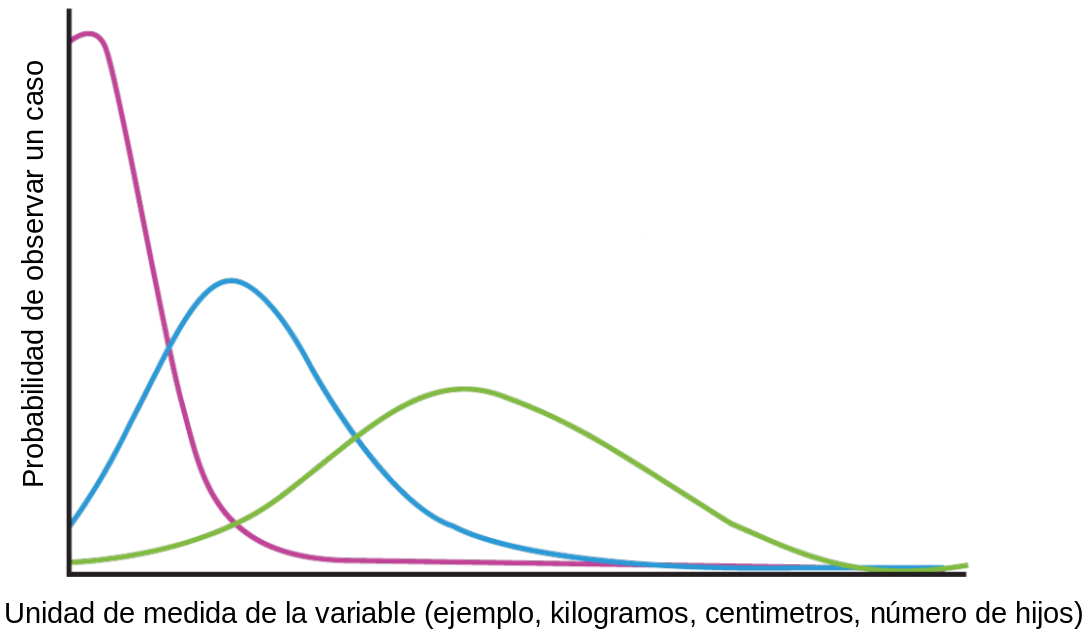
\includegraphics[width=.75\textwidth]{estudiar.png}
\end{figure}
\end{frame}

\begin{frame}
Primero, debemos entender el concepto de \textbf{caso, observación, o registro}. La colección de casos es lo que se llama \textbf{distribución estadística}.
\begin{figure}
\centering
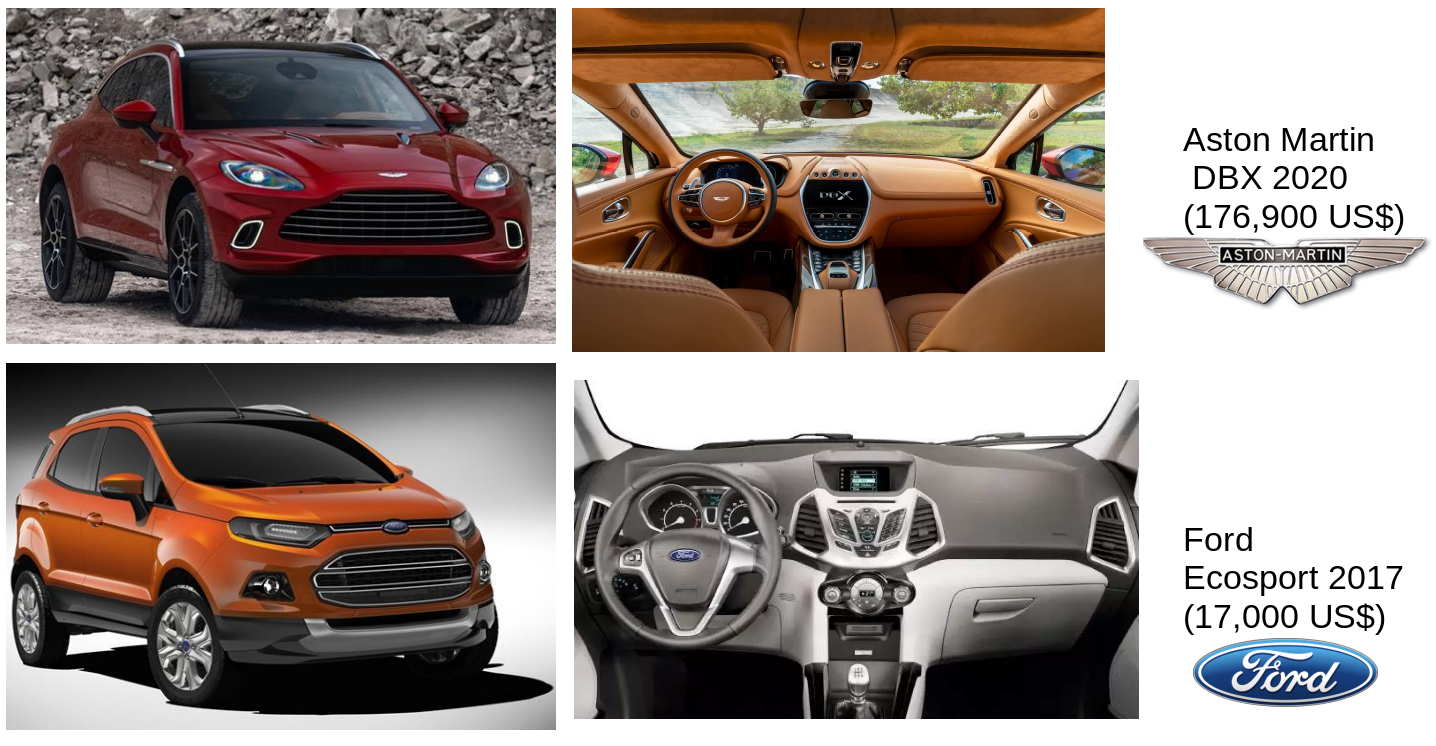
\includegraphics[width=.65\textwidth]{casos.png}
\end{figure}
Sin una distribución estadística es muy difícil afirmar ideas tales como cuál de estos dos vehículos es ``\textit{normal o típico}''
\end{frame}

\begin{frame}
En analítica de datos, el interés siempre recae en analizar datos para extraer información a partir de ellos, y deducir conocimiento útil a partir de la información que extraigamos de los datos.\\
\vspace{0.5cm}
Entender cómo se describe una distribución estadística es, probablemente, lo más fundamental para un experto en analítica de datos. Para entender cómo describirla, es imprescindible apoyarse en tres características fundamentales: \textbf{tendencia}, \textbf{variación} y \textbf{forma}.
\end{frame}

\begin{frame}
\begin{itemize}
\item \textbf{Tendencia}: Es la característica de una distribución estadística que se refiere al punto en el que se observan mayor frecuencia de casos u observaciones. La tendencia se mide a través de indicadores como \textbf{promedio}, \textbf{mediana} o \textbf{moda}.
\vspace{0.2cm}
\item \textbf{Variación}: Se refiere al conjunto de observaciones que definen los límites inferiores y superiores dentro de los cuales se observan los casos. La variación de una distribución se mide con indicadores como la \textbf{desviación estándar}, la \textbf{varianza} o el \textbf{rango intercuartilar}
\vspace{0.2cm}
\item \textbf{Forma}: Se refiere a la apariencia visual que adopta una colección de casos u observaciones luego de ordenarlos con base en algún criterio. La forma de una distribución se mide con indicadores como la \textbf{asimetría} y la \textbf{curtosis}.
\end{itemize}    
\end{frame}


\begin{frame}
\begin{figure}
\centering
\includegraphics[width=.85\textwidth]{estudiemos.pdf}
\end{figure}
\end{frame}


\begin{frame}
Si usted abre el jupyter notebook del capítulo 1 del libro de \citeauthor{Molin2021} \citeyear{Molin2021} observará con detalle computacional cómo se hacen los cálculos.
\begin{figure}
\centering
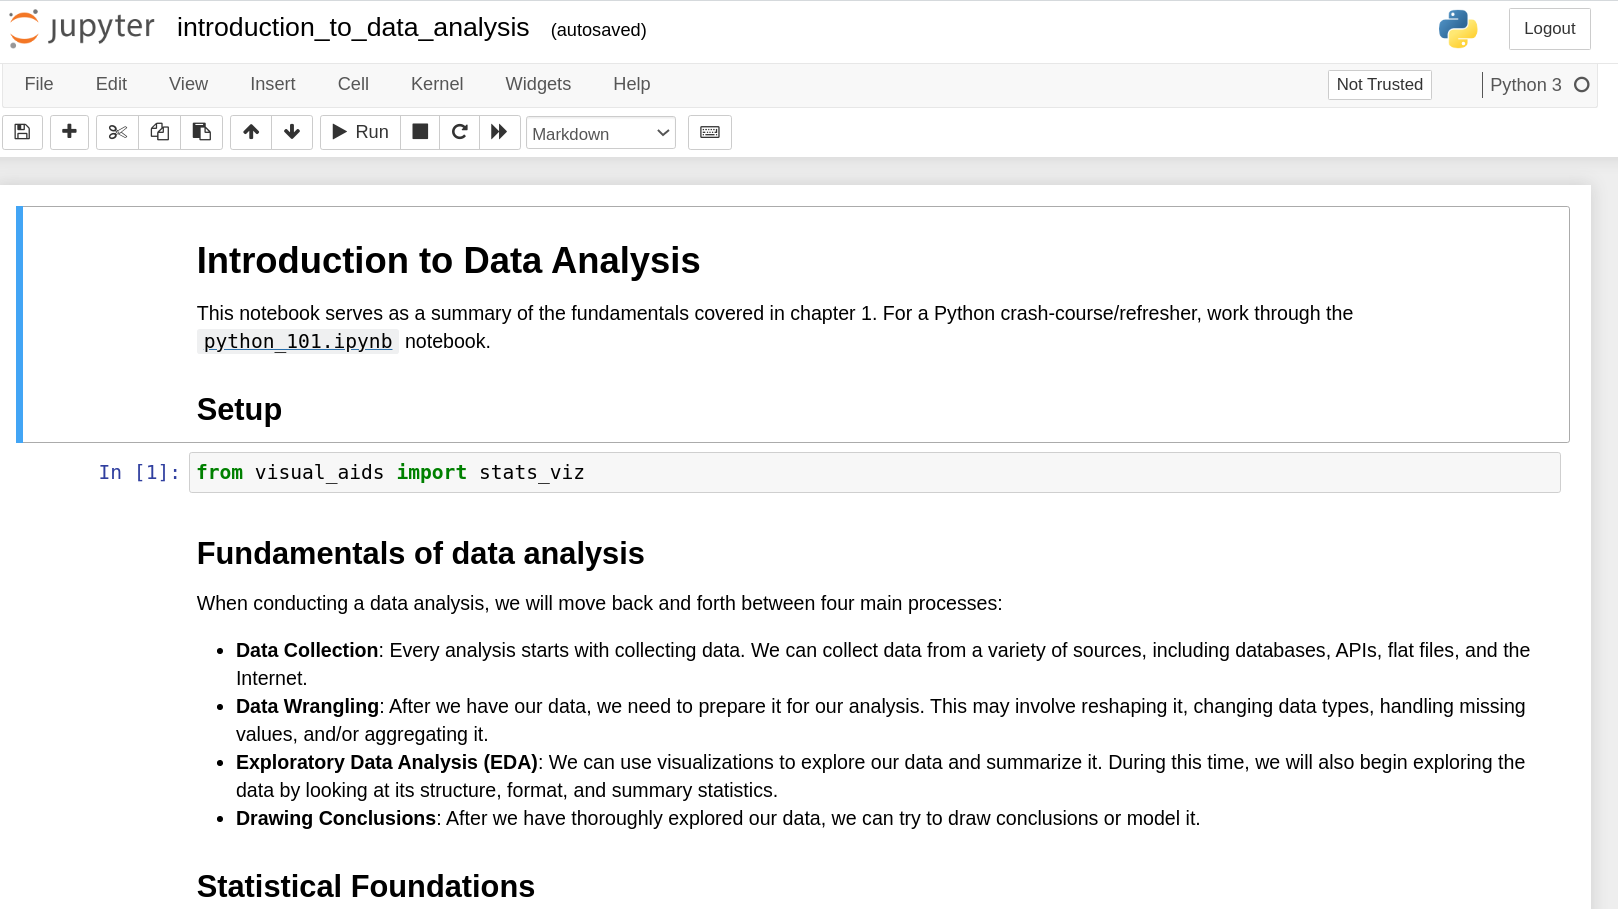
\includegraphics[width=.65\textwidth]{c1.png}
\end{figure}
\end{frame}

\begin{frame}
Ejercicio Guiado:
\vspace{0.5cm}
\begin{itemize}
\item Abrir el jupyter notebook del capítulo 1 del libro de \citeauthor{Molin2021} \citeyear{Molin2021}.
\item Intentar reproducir las sintaxis que aparecen en ese jupyter notebook.
\end{itemize}
\begin{figure}
\centering
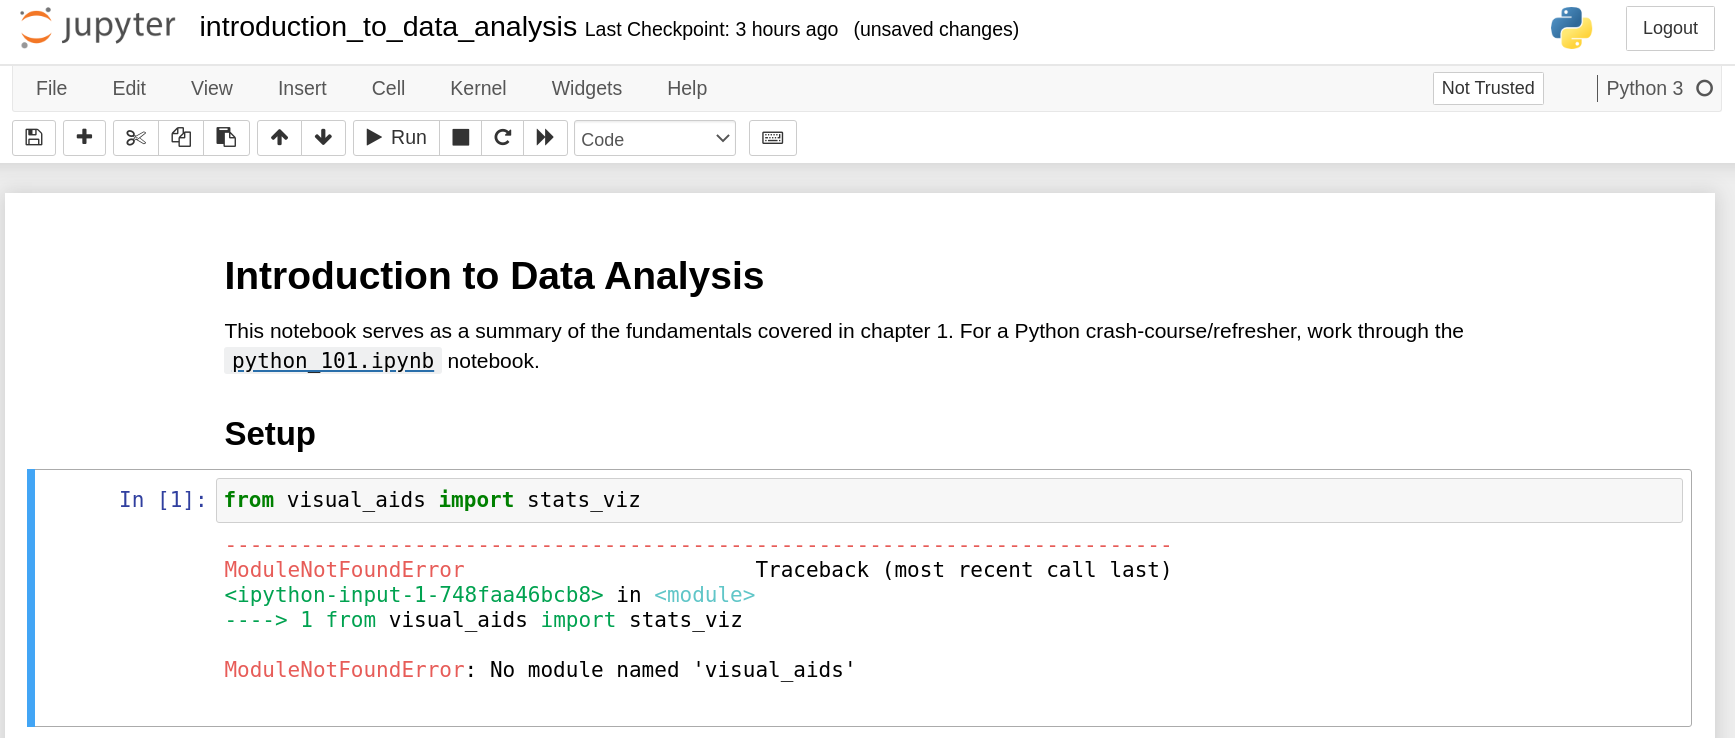
\includegraphics[width=.65\textwidth]{problema.png}
\end{figure}
\centering
¿Le aparece este problema?
\end{frame}

\begin{frame}
Observe lo que \citeauthor{Molin2021} \citeyear{Molin2021} comenta en la página 5 del capítulo 1.
\begin{figure}
\centering
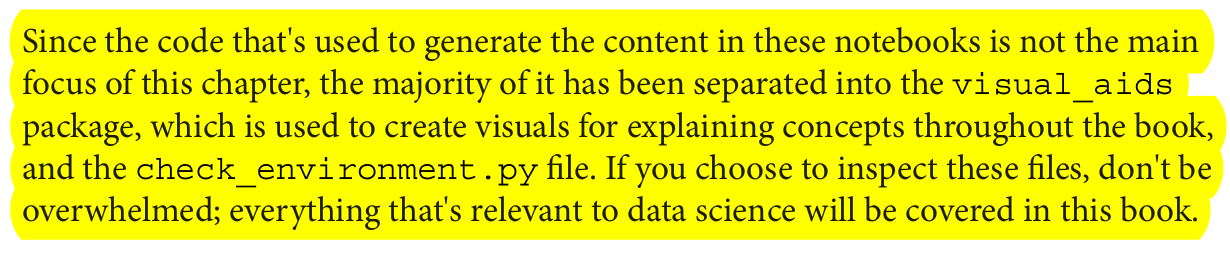
\includegraphics[width=.75\textwidth]{instrucciones.png}
\end{figure}
Para chequear las librerías o paquetes de software que se requieren para ejecutar las sintaxis en el jupyter notebook llamado \texttt{introduction\_to\_data\_analysis}, basta con abrir la terminal de su computador, cambiar de directorio (Carpeta GitHub) y escribir el siguiente código o sintaxis\\
\begin{center}
\texttt{python3 check\_environment.py}    
\end{center}
\end{frame}

\begin{frame}
Debería aparecerle algo así como lo siguiente
\begin{figure}
\centering
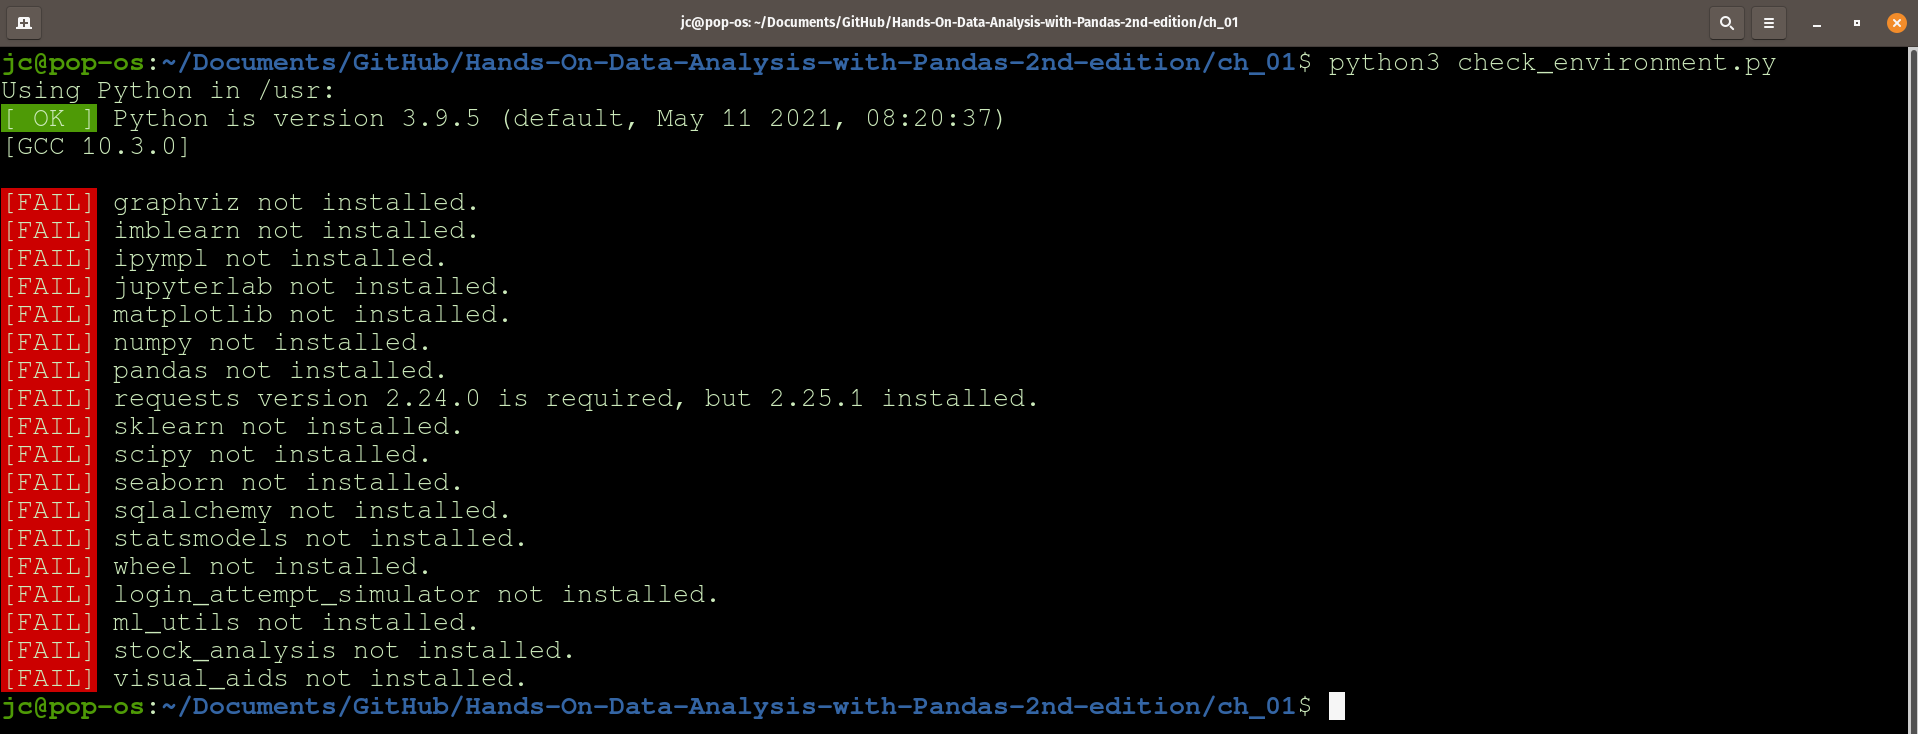
\includegraphics[width=.95\textwidth]{problemas.png}
\end{figure}
(No se preocupe si observa alguna diferencia en la apariencia de este pantallazo con relación a lo que usted observa en su computador).
\end{frame}

\begin{frame}
Por ahora, nos interesa comprender cómo, a partir del concepto de distribución estadística, se entiende el concepto de \textbf{análisis de varianza}.   
\begin{figure}
\centering
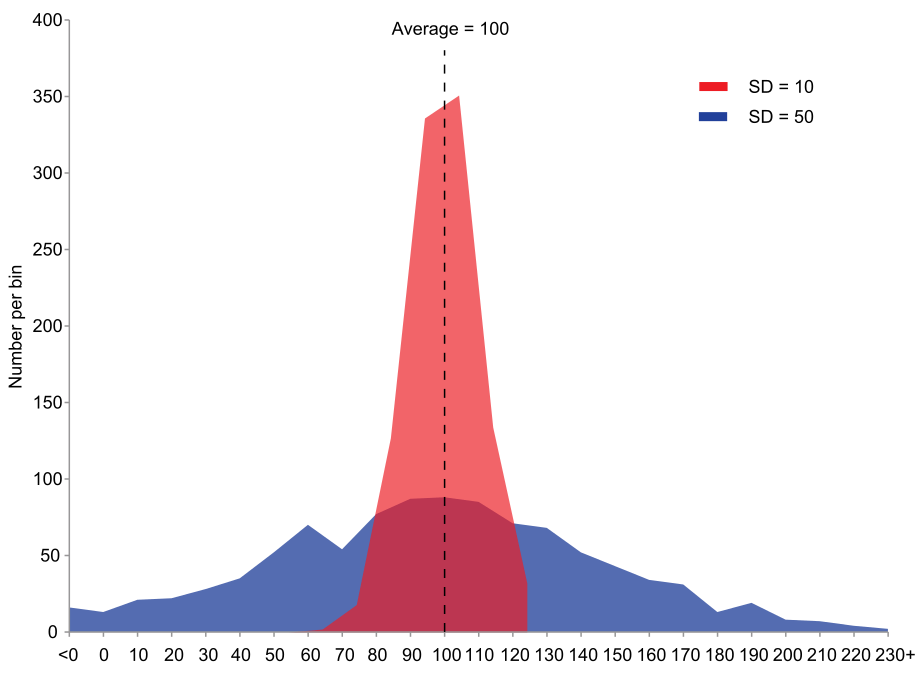
\includegraphics[width=.32\textwidth]{sd.png}
\end{figure}
La \textbf{varianza} indica cuánto cambian o varían los casos de la distribución. Visualmente puede entenderse cómo cuán ancha o estreche es la base de una distribución. La varianza se calcula como el cuadrado de la desviación estándar (SD). En la imagen, la distribución roja tiene menos varianza que la azul, aunque ambas tienen exactamente el mismo promedio.
\end{frame}

\begin{frame}
El análisis de la varianza (o ANOVA: ``\textit{Analysis of variance}'' como se le dice en inglés) es una técnica estadística que sirve para comprender las diferencias del promedio entre tres o más \textbf{grupos metodológicamente comparables}.\\
\vspace{0.5cm}
Dos o más grupos son \textbf{metodológicamente comparables} si pertenecen conceptual o empíricamente al mismo universo o población. \\
\vspace{0.5cm}
Por ejemplo, los estudiantes de la universidad de Los Andes y del CESA son metodológicamente comparables porque ambos grupos pertenecen a la población de instituciones de educación superior en Colombia. Los estudiantes del CESA y los de la Universidad de Hiroshima no son metodológicamente comparables.
\end{frame}

\begin{frame}
Para interpretar los resultados de un ANOVA, hay que entender si las distribuciones de los grupos son o no diferentes desde el punto de vista probabilístico.\\
\vspace{0.5cm}
Conceptualmente, las diferencias probabilísticas no son iguales a las diferencias matemáticas.\\
\vspace{0.5cm}
En matemáticas, el número 3 es estrictamente hablando diferente del número 2.999. En probabilidades, sin embargo, podría asumirse tranquilamente que ambos números podrían ser iguales desde el punto de vista probabilístico.\\
\vspace{0.5cm}
¿Entonces, en qué podemos apoyarnos para decir si dos números son o no iguales desde el punto de vista probabilístico?
\end{frame}

\begin{frame}
\begin{figure}
\centering
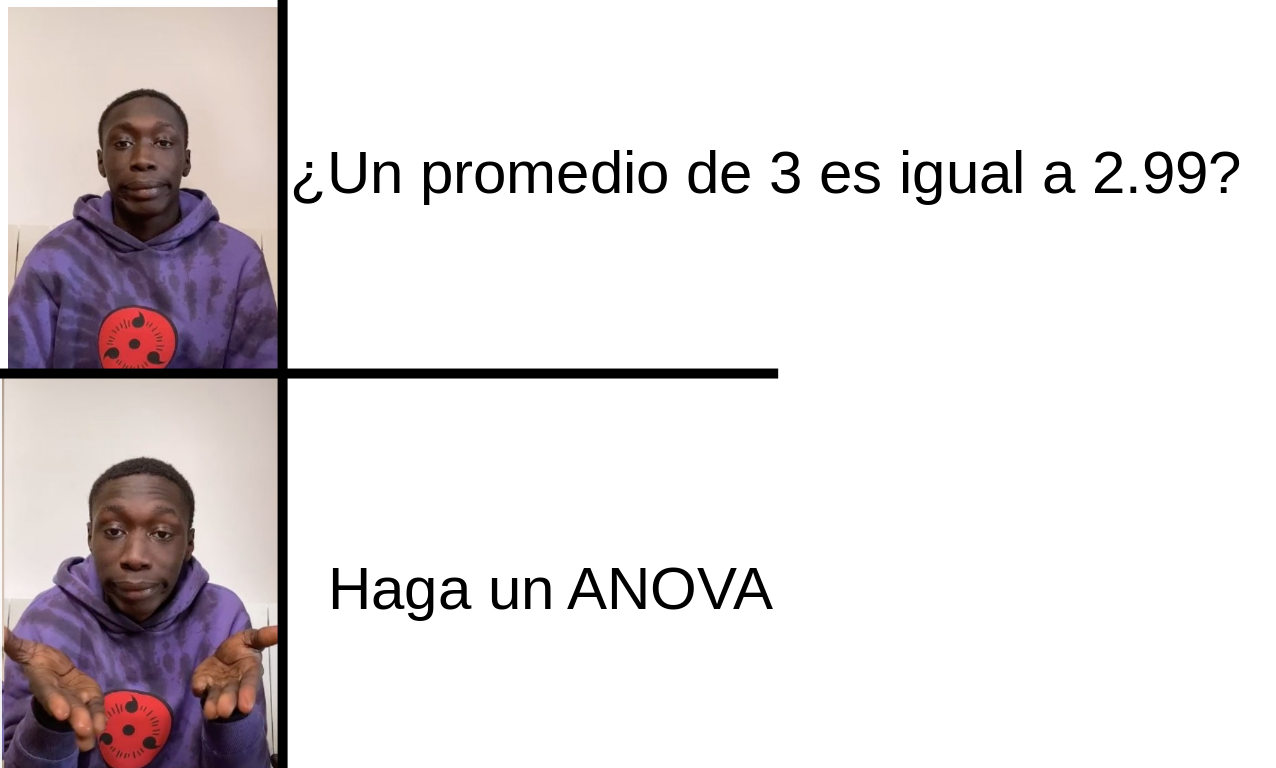
\includegraphics[width=.75\textwidth]{lame.png}
\end{figure}
\end{frame}

\begin{frame}
Desde el punto de vista de cálculo, un ANOVA genera como resultado un conjunto de información referente a las diferencias probabilísticas de tres o más grupos. 
\begin{figure}
\centering
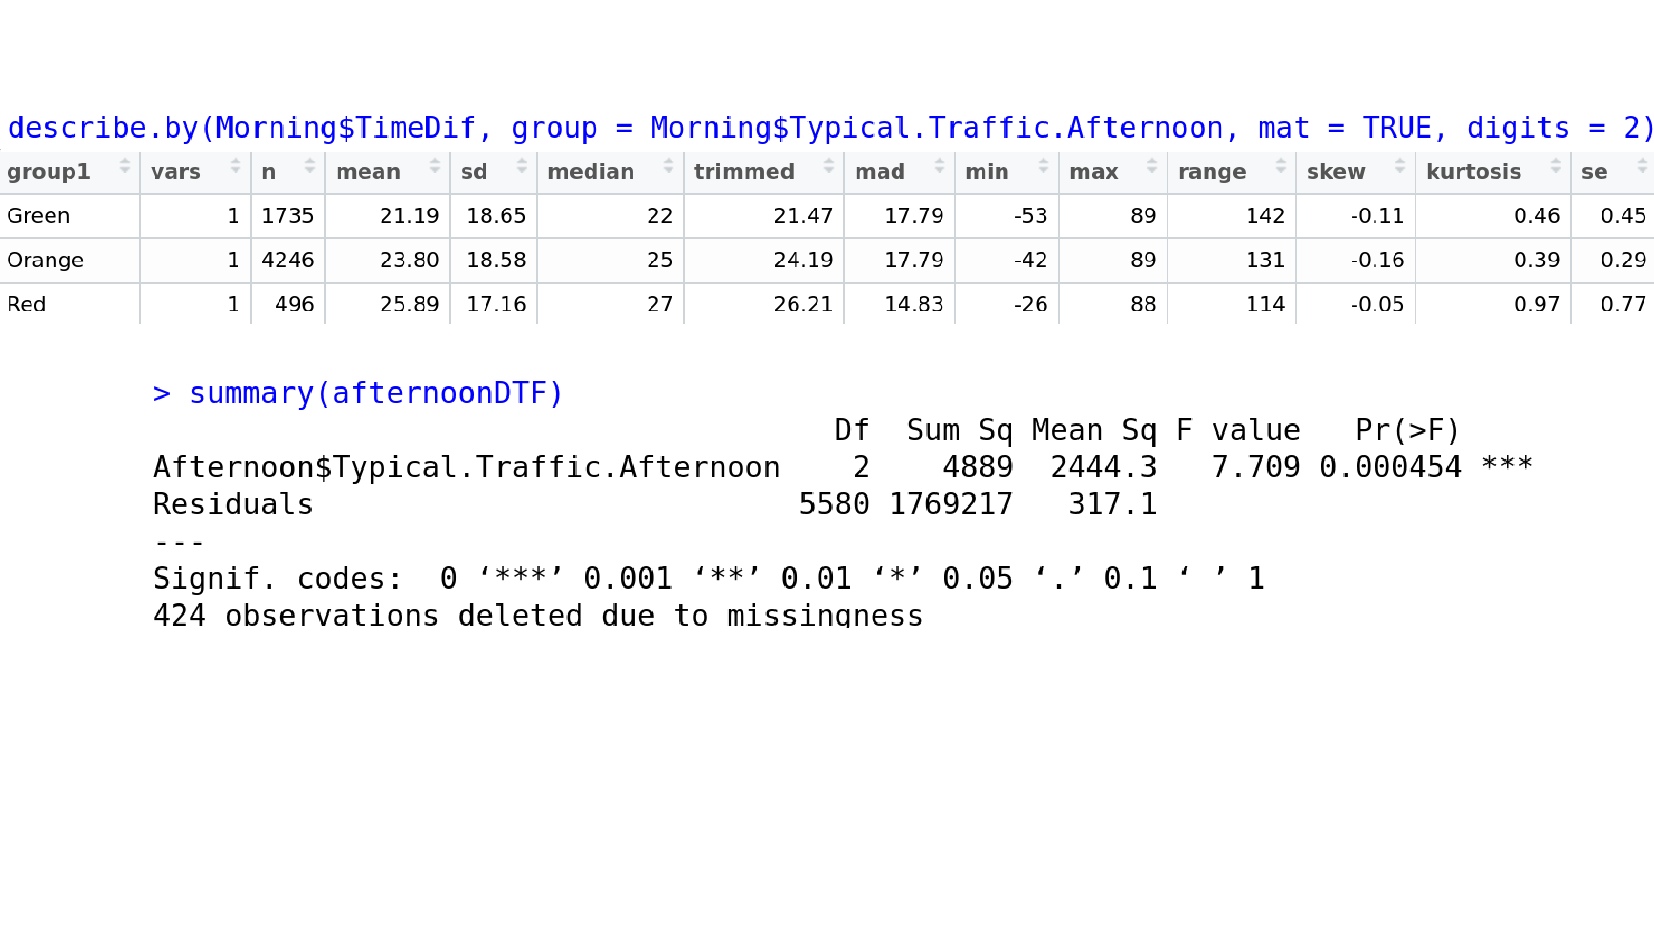
\includegraphics[width=.75\textwidth]{resultados.pdf}
\end{figure}
\end{frame}

\begin{frame}
Visualmente, las diferencias entre tres o más grupos son estadísticamente significativas si sus distribuciones se separan entre sí.
\begin{figure}
\centering
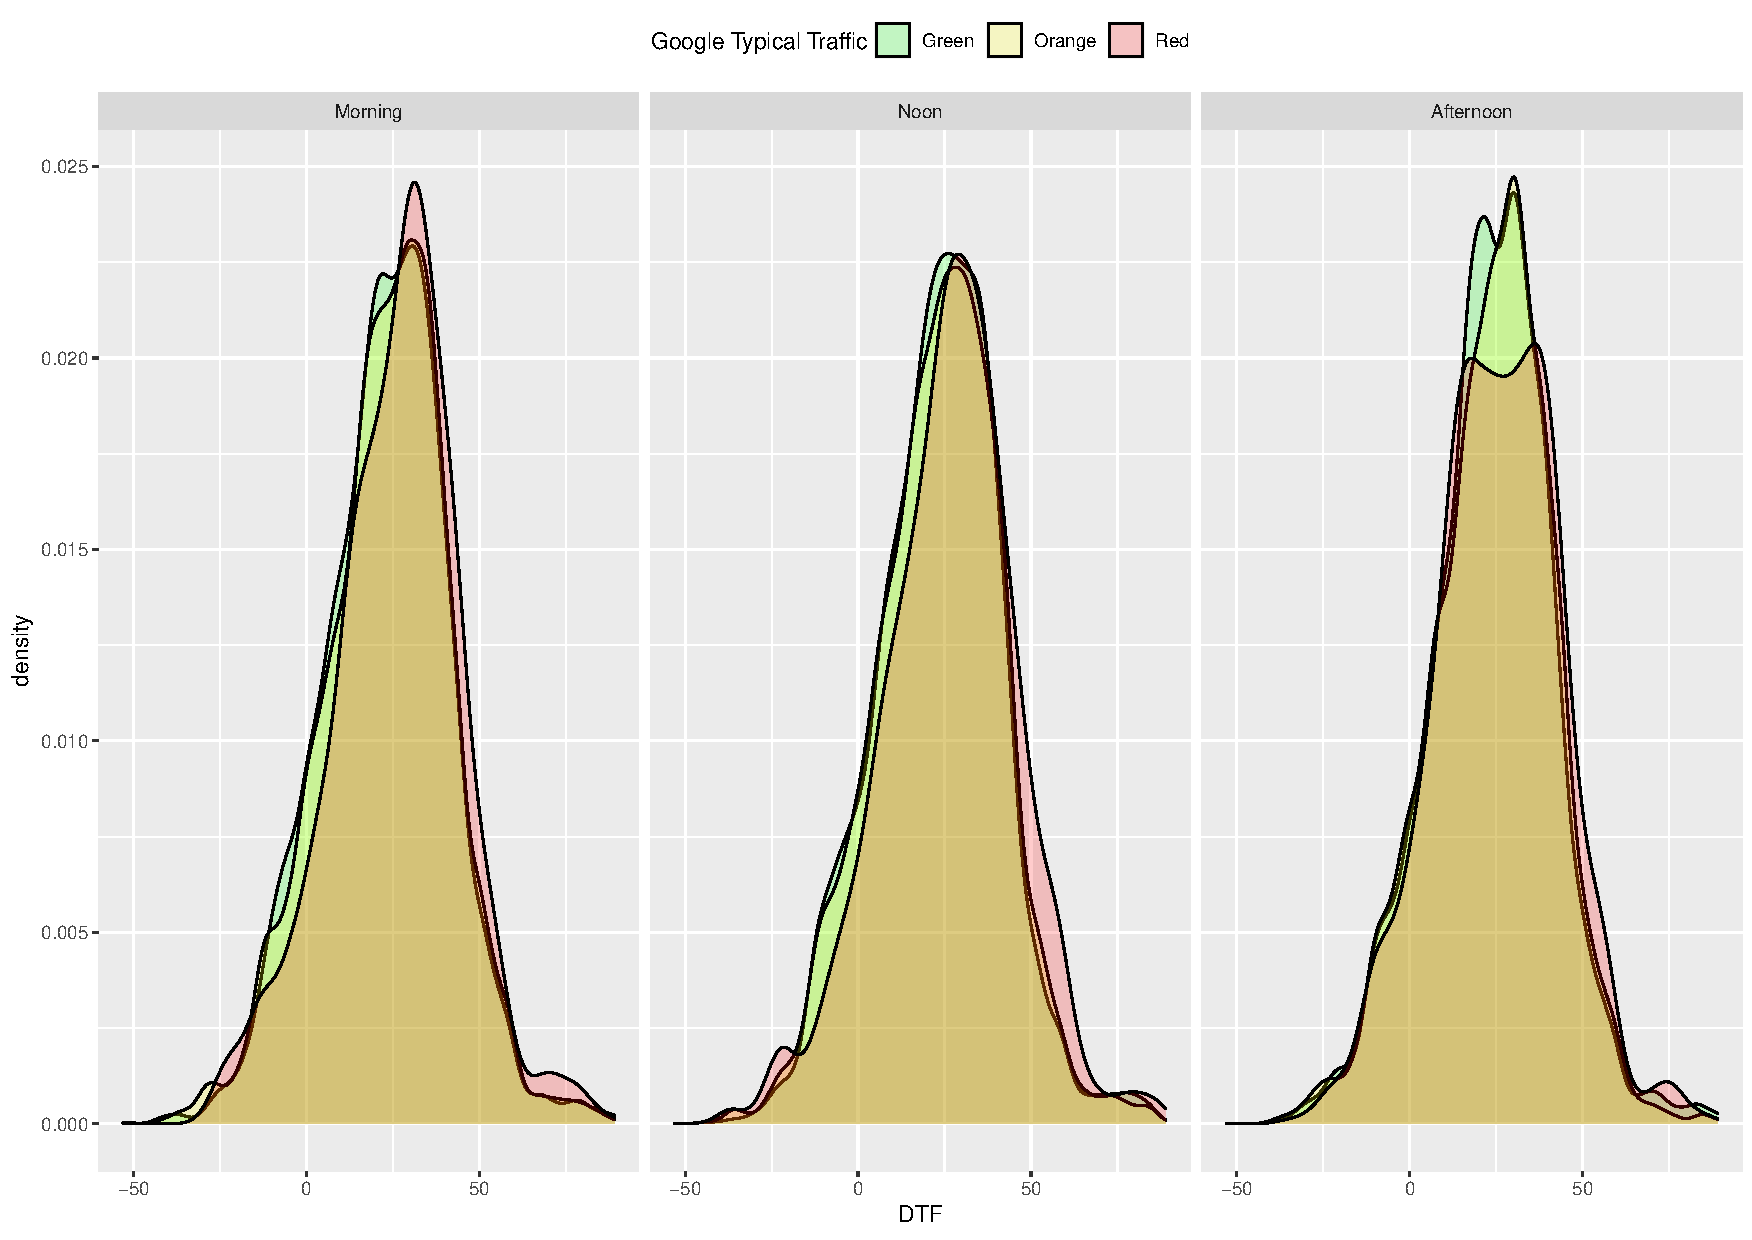
\includegraphics[width=.4\textwidth]{Rplot.pdf}
\end{figure}
Este gráfico se obtuvo luego de llegar a la línea 102 de nuestro repo de GitHub, correspondiente al artículo de domicilios de comida en Bogotá \cite{Correa2019}.
\end{frame}



\section*{REFERENCIAS}
\begin{frame}[allowframebreaks]{Referencias}
\tiny{ 
\bibliographystyle{apacite}
\bibliography{REFS.bib}
} 
\end{frame}

\setbeamertemplate{background}{\tikz[overlay,remember picture]\node[opacity=1]at (current page.center){
\includegraphics[width=18cm]{ulam.png}};}
\pgfdeclareimage[height=0cm,width=0cm]{}{}
 \logo{\pgfuseimage{}}
\beamertemplatenavigationsymbolsempty
\begin{frame}
\end{frame}
\end{document}